\documentclass[14pt]{extarticle}

% Общие пакеты
\usepackage[utf8]{inputenc}
\usepackage[T2A]{fontenc}
\usepackage[russian]{babel}

% Математические пакеты
\usepackage{amsmath, amssymb, amsthm, mathrsfs}

% Пакеты для формата страницы
\usepackage[a4paper,margin=2.5cm]{geometry}
\usepackage[notlof,notlot]{tocbibind}
\usepackage{needspace}

\usepackage{titlesec, enumitem}

% Каждая секция начинается с новой страницы
\titleformat{\section}
  {\clearpage\normalfont\Large\bfseries}{\thesection}{1em}{}

% Устанавливаем отступы
\setlength{\parindent}{0pt}

\titlespacing{\subsection}{0pt}{4\baselineskip}{1\baselineskip}
\titlespacing{\subsubsection}{0pt}{2\baselineskip}{1\baselineskip}

% Отступы для текста
\clubpenalty=10000          % Запрет одиночных строк в начале страницы
\widowpenalty=10000         % Запрет одиночных строк в конце страницы
\displaywidowpenalty=10000  % То же для формул
\brokenpenalty=10000        % Запрет переносов в неподходящих местах
\tolerance=1000             % Допустимая растяжимость строк
\emergencystretch=3pt       % Экстренная растяжимость

% Минимальное количество строк для переноса абзаца
\raggedbottom              % Позволяет страницам быть разной высоты
\setlength{\parfillskip}{0pt plus 1fil}

% Настройки для предотвращения разрывов коротких абзацев
\newcommand{\needparagraph}[1]{
    \needspace{3\baselineskip}
    #1
}

% Настройки для секций (чтобы заголовки не "висели" в одиночестве)
\titlespacing{\section}{0pt}{3\baselineskip plus 1\baselineskip}{1\baselineskip}
\titlespacing{\subsection}{0pt}{4\baselineskip}{1\baselineskip}
\titlespacing{\subsubsection}{0pt}{2\baselineskip}{1\baselineskip}

% Отступы для списков
\setlist[enumerate]{noitemsep, topsep=0pt}
\setlist[itemize]{noitemsep, topsep=0pt}

\let\olditem\item
\renewcommand{\item}{\needspace{2\baselineskip}\olditem}

% Глубина нумерации
\setcounter{secnumdepth}{3}
\setcounter{tocdepth}{3}

% Ссылки
\usepackage{hyperref, cleveref}

% Цвета для блоков
\usepackage{tcolorbox, xcolor}
\definecolor{theoremcolor}{HTML}{F0F0F0}
\definecolor{bordercolor}{HTML}{708090}
\usepackage{fancyhdr}
\pagestyle{fancy}

% Устанавливаем рекомендуемую высоту заголовка
\setlength{\headheight}{17.0pt}
\addtolength{\topmargin}{-2.5pt}

\fancyhf{} % очистить все поля

% Верхний колонтитул: название и номер секции
\fancyhead[L]{\nouppercase{\leftmark}}
\fancyhead[R]{\thepage}

% Нижний колонтитул
\fancyfoot[C]{\textit{}}

\renewcommand{\headrulewidth}{0.4pt}
\renewcommand{\footrulewidth}{0.4pt}

% Подключаем tcolorbox
\tcbuselibrary{theorems,skins,breakable}

% Стиль рамки для теорем
\tcbset{theostyle/.style={
  colback=theoremcolor!50,
  colframe=bordercolor,
  fonttitle=\bfseries,
  coltitle=black,
  boxrule=0.8pt,
  arc=2mm,
  left=1.5mm,
  right=1.5mm,
  top=1mm,
  bottom=1mm,
  enhanced,
  breakable,
  before skip=\baselineskip,
  after skip=\baselineskip
}}

% Определения новых теорем
\newtcbtheorem[auto counter, number within=section]{theorem}{Теорема}{theostyle}{th}
\newtcbtheorem[auto counter, number within=section]{lemma}{Лемма}{theostyle}{lem}
\newtcbtheorem[auto counter, number within=section]{definition}{Определение}{theostyle}{def}
\newtcbtheorem[auto counter, number within=section]{example}{Пример}{theostyle}{ex}

\title{Вычмат-2025}

\begin{document}

\maketitle
\tableofcontents

\section{Основные определения}

\subsection{Предмет вычислительной математики. Метод и задачи вычислительной математики в терминах функционального анализа.}

    \subsubsection{Предмет вычислительной математики.}

        Необходимость разработки методов доведения математических исследований до числового результата привела к созданию отдельной дисциплицы - \textbf{вычислительной математики}.

        \begin{definition}{Вычислительная математика-1}{def-compmath-1}
            Область математики, которая призвана разрабатывать методы доведения до числового результата решений основных задач математического анализа, алгебры и геометрии и пути использования для этой цели современных вычислительных средств.
        \end{definition}

        \begin{definition}{Вычислительная математика-2}{def-compmath-2}
            Раздел математики, связанный с построением и анализом алгоритмов численного решения математических задач.
        \end{definition}

        Таким образом, \textbf{вычислительная математика} помогает решать численные задачи с помощью ЭВМ.

    \subsubsection{Функциональный анализ.}
        \begin{definition}{Функциональный анализ}{def-func-analysis}
            Область математики, изучающая свойства функциональных пространств.
        \end{definition}

        Для определения \textbf{задач и методов} вычислительной математики введем важнейшие \textbf{понятия функционального анализа}.

        \begin{definition}{Понятия функционального анализа}{def-func-analysis}
            \begin{itemize}
                \item Функциональные метрические пространства.
                \item Функции, определенные на функциональных пространствах.
            \end{itemize}
        \end{definition}

        \textbf{Функциональный анализ} рассматирвает элементы более общего (не евклидова) пространства.

    \subsubsection{Функциональные метрические пространства.}
        
        В функциональном анализе вместо евклидовых пространств рассматриваются абстрактные пространства, элементы которых могут иметь самую различную природу.

        \begin{definition}{Метрическое пространство}{def-metric-space}
            Абстрактное множество, для любых двух элементов $x$ и $y$ которого \textbf{опрделено} понятие \textbf{расстояния} $\rho(x, y)$.
        \end{definition}

        \begin{lemma}{Свойства расстояния}{lem-distance-features}
            \textbf{Расстояние} $\rho(x, y)$ должно удовлетворять следующим \textbf{свойствам:}
            \begin{enumerate}
                \item $\rho(x,y) \geq 0$, причем $\rho(x, y) = 0$ $\leftrightarrow$ $x$ совпадает с $y$.
                \item $\rho(x, y) = \rho(y, x)$.
                \item $\rho(x, y) \leq \rho(x, z) + \rho(z, y)$ $\forall$ $x, y, z \in \mathscr{R}$, где: $\mathscr{R}$ - метрическое пространство.
            \end{enumerate}
        \end{lemma}

        Евклидовы пространства с обычным определением расстояния удовлетворяют всем этим условиям. Но могут быть и другие метрические пространства.

        \begin{definition}{Пространство непрерывных функций}{def-continuous-func-space}
            Пространство $C[a, b]$ - множество всех непрерывных функций на отрезке $[a, b]$.\\
            Функция $f(x)$ непрерывная на $[a, b]$ $\leftrightarrow$ $f(x) \in C[a, b]$.
        \end{definition}

        \begin{example}{Неевклидово метрическое пространство}{ex-noneuclidean-metric-space}
            Пространства $L_{p}$, где $p \geq 1$ и $p \in \mathbb{R}$.
            $$L_{p} = \{f(x) \text{| } f(x) \in \text{C}[a, b] \text{, } \int_{a}^{b}|f(t)|^{p} \, dt < \infty\}$$

            Расстояние $\rho(x, y)$ в пространстве $L_{p}$ определяется следующим образом:
            $$\rho(x, y) = [\int_{a}^{b}|x(t) - y(t)|^{p}]^{\frac{1}{p}}$$
        \end{example}

        В каждом метрическом пространстве можно говорить об \textbf{окрестности данной точки}.

        \begin{definition}{Окрестность точки}{def-point-locality}
            $\varepsilon$-окрестностью точки $x$ некоторого метрического пространства $\mathscr{R}$ называется множество точек $y$ таких, что:
            $$\rho(x, y) \leq \varepsilon$$
        \end{definition}

        \begin{example}{Окрестность точки в $L_{p}$}{ex-point-locality}
            Окрестность точки в $L_{p}$ - это совокупность всех функций $y(t)$, принадлежащих $L_{p}$, для которых:
            $$\int_{a}^{b} |x(t) - y(t)|^{p} \, dt < \varepsilon^{p}$$
        \end{example}

        В вычислительной математике часто приходится заменять одну функцию $x(t)$ другой, более удобной для вычислительных целей. Обычно эту вторую функцию берут из $\varepsilon$-окрестности первой.

    \subsubsection{Функции, заданные на функциональном пространстве.}
        
        \begin{definition}{Операторы функционального пространства}{def-operator}
            Пусть нам даны два абстрактных (функциональных) пространства $\mathscr{R}_{1}$ и $\mathscr{R}_{2}$ и каждому элементу $x \in \mathscr{R}_{1}$ поставлен в соответствие элемент $y \in \mathscr{R}_{2}$. Тогда будем говорить, что нам задан \textbf{оператор}:
            $$y = A(x)$$
            с областью определения $\mathscr{R}_{1}$ и областью значений, принадлежащих $\mathscr{R}_{2}$.

            \vspace{\baselineskip}

            В частности, если $\mathscr{R}_{2}$ является областью вещественных или комплексных чисел, то оператор $A(x)$ - \textbf{функционал}.
        \end{definition}

        \begin{example}{Функционал}{ex-operator}
            Оператором (функционалом) в пространстве непрерывных функций на отрезке $[a, b]$ $C[a, b]$ - \textbf{определенный интеграл}:
            $$I(x) = \int_{a}^{b} x(t) \, dt$$
        \end{example}

    \subsubsection{Методы и задачи вычислительной математики.}

        \begin{definition}{Задачи вычислительной математики}{def-compmath-problems}
            Многие задачи в вычислительной математике могут быть записаны в виде:
            $$y = A(x)$$
            где $x$ и $y$ принадлежат заданным пространствам $\mathscr{R}_{1}$ и $\mathscr{R}_{2}$ и $A(x)$ - некоторых заданный оператор.
        \end{definition}

        Далеко не всегда с помощью средств современной математики удается точно решить эти задачи, применяя конечное число шагов. Для этого используют \textbf{методы вычислительной математики}:

        \begin{definition}{Основной метод вычислительной математики}{def-compmath-main-method}
            Замена пространств $\mathscr{R}_{1}$ и $\mathscr{R}_{1}$ и $\mathscr{R}_{2}$ и оператора $A(x)$ другими пространствами $\overline{\mathscr{R}_{1}}$ $\overline{\mathscr{R}_{2}}$ и оператором $\overline{A}$, более удобными для вичислительных целей.
            Замена $\overline{y} = \overline{A(\overline{x})}$ должна удовлетворять следующим неравенствам:
            $$\rho(x, \overline{x}) < \varepsilon$$
            $$\rho(y, \overline{y}) < \varepsilon$$
        \end{definition}

        Иногда бывает достаточно произвести замену только пространств $\mathscr{R}_{1}$ и $\mathscr{R}_{2}$ или даже одного из них, или заменить только оператор.

        \begin{example}{Применение метода}{ex-method-application}
            $f(x) \in C[a, b]$. Требуется решить задачу:
            $$y = \int_{a}^{b} f(x) \, dx$$
            причем интеграл не берется в элементарных функциях.

            Тогда возможны два пути:
            \begin{enumerate}
                \item \textbf{Замена пространств:} вместо $f(x)$ взять $P_{n}(x)$ - алгебраический многочлен степени $n$.
                \item \textbf{Замена оператора:} вместо интегрирования построить интегральную сумму $\sum_{i=1}^{n}f(x_{i})\Delta_{i}$.
            \end{enumerate}
        \end{example}

        \begin{definition}{Вычислительный метод}{def-comp-method}
            Метод, используемый для преобразования задач к виду, удобному для реализации на ЭВМ.
        \end{definition}

        \begin{definition}{Основные вычислительные методы}{def-main-comp-methods}
            \textbf{Основные классы} вычислительных методов:
            \begin{itemize}
                \item \textbf{Методы эквивалентных преобразований} (замена исходной задачи другой (более простой), имеющее то же решение).
                \item \textbf{Методы аппроксимации} (аппроксимировать исходную задачу другой с небольшой погрешностью решения).
                \item \textbf{Итерационные методы} (через итерационные последовательности и функции).
            \end{itemize}

        \end{definition}

        Резюмируя, можно выделить \textbf{основные задачи} вычислительной математики:

        \begin{example}{Основные задачи}{ex-main-compmath-problems}
            \begin{itemize}
                \item Приближение множеств в функциональных пространствах.
                \item Приближение операторов, заданных на функциональных пространствах.
                \item Разработка рациональных алгоритмов и методов решения задач в условиях приминения современных вычислительных средств.
            \end{itemize}
        \end{example}

\clearpage
\subsection{Источники и классификация погрешностей результатов численного решения задач. Приближенные числа. Абсолютная и относительная погрешности. Правила записи приближенных чисел.}

    \subsubsection{Источники и классификация погрешностей}

        При решении прикладной задачи с использованием ЭВМ получить точное решение задачи практически невозможно. Получаемое \textbf{решение} почти \textbf{всегда содержит погрешность}, т.е. является приближенным. 
        \begin{definition}{Источники погрешности решения}{def-error-sources}
            Пусть y - точное значение величины, а $y^{*}$ - ее приближенное значение, тогда:
            
            \begin{enumerate}
                \item \textbf{Неустранимая погрешность:} $\delta_{\text{н}}y^{*}$ - математическая модель и исходные данные вносят в решение ошибку, которая не может быть устранена далее.
                \item \textbf{Ошибка метода решения:} $\delta_{\text{м}}y^{*}$ - источник данной погрешности - метод решения задачи.
                \item \textbf{Вычислительная погрешность:} $\delta_{\text{в}}y^{*}$ - определяется характеристикой машины ЭВМ.
            \end{enumerate}
        \end{definition}

        Таким образом, полная погрешность результата решения задачи на ЭВМ складывается из трех составляющих:
        $$\delta y^{*} = \delta_{\text{н}}y^{*} + \delta_{\text{м}}y^{*} + \delta_{\text{в}}y^{*}$$

        \textbf{На практике} исходят из того, что: 
        \begin{itemize}
            \item Погрешность метода должна быть на порядок меньше неустранимой погрешности.
            \item Величина вычислительной ошибки была хотя бы на порядок меньше величины погрешности метода.
        \end{itemize}

    \clearpage
    \subsubsection{Приближенные числа. Абсолютная и относительная погрешности.}
        
        Пусть $а$ - точное (неизвестное) значение некоторой величины, $a^{*}$ - приближенное (известное) значение той же величины (приближенное число).

        \begin{definition}{Абсолютная погрешность}{def-absolute-error}
            Модуль разности приближенного и точного значения некоторой величины:
            $$\Delta(a^{*}) = |a - a^{*}|$$
        \end{definition}

        \begin{definition}{Относительная погрешность}{def-relative-error}
            Для соотншения погрешность величины и ее значения вводят понятие \textbf{относительной погрешности}:
            $$\delta(a^{*}) = \frac{|a - a^{*}|}{|a|} = \frac{\Delta(a^{*})}{|a|}$$
        \end{definition}

        Т.к. значение $а$ неизвестно, то непосредственное вычисление величин $\Delta(a^{*})$ и $\delta(a^{*})$ по предыдущим формулам невозможно, то вводят верхние границы погрешностей.

        \begin{definition}{Верхние границы погрешностей}{def-upper-limits-error}
            $\overline{\Delta(a^{*})}$ и $\overline{\delta(a^{*})}$ - верхние границы абсолютной и относительной погрешностей соответственно:
            $$|a - a^{*}| \leq \overline{\Delta(a^{*})}$$
            $$\frac{|a - a^{*}|}{|a|} \leq \overline{\delta(a^{*})}$$

            Причем, если величина $\overline{\Delta(a^{*})}$ известна, то:
            $$\overline{\delta(a^{*})} = \frac{\overline{\Delta(a^{*})}}{|a|}$$

            Аналогично, если известна $\overline{\delta(a^{*})}$:
            $$\overline{\Delta(a^{*})} = |a| \cdot \overline{\delta(a^{*})}$$            
        \end{definition}

    \subsubsection{Правила записи приближенных чисел.}
        
        Пусть приближенное число $a^{*}$ задано следующим образом:
        $$a^{*} = \alpha_{n}\alpha_{n-1}\ldots\alpha_{0}.\beta_{1}\beta_{2}\ldots\beta_{m}$$
        где $\alpha_{n}\alpha_{n-1}\ldots\alpha_{0}$ - целая часть, $\beta_{1}\beta_{2}\ldots\beta_{m}$ - дробная.

        \begin{definition}{Значащие цифры}{def-significant-digits}
            Все цифры в записи числа $a^{*}$, начиная с первой ненулевой слева.
        \end{definition}

        \begin{definition}{Верная цифра}{def-correct-digit}
            Значащую цифру называют \textbf{верной}, если абсолютная погрешность числа не превосходит единицы разряда, соответствующей этой цифре.
        \end{definition}

        \begin{example}{Значащие и верные цифры}{ex-significant-and-correct-digits}
            Пусть $a^{*} = 0.010300$, $\Delta(a^{*}) = 2 \cdot 10^{-6}$:
            
            \begin{enumerate}
                \item \textbf{Значащие цифры:} $10300$
                \item \textbf{Верные цифры:} $1030$
            \end{enumerate}
        \end{example}

        \begin{lemma}{Связь числа верных цифр с отностительной погрешностью}{lem-relative-correct-connection}
            Если число $a^{*}$ имеет ровно $N$ верных цифр, то $\delta(a^{*}) \sim 10^{-N}$.
        \end{lemma}

        \begin{lemma}{Правило записи}{lem-note-rule}
            Неравенство верхней границы абсолютной погрешности эквивалентно следующему:
            $$a^{*} - \overline{\Delta{a^{*}}} \leq a \leq a^{*} + \overline{\Delta{a^{*}}}$$
            
            Тот факт, что число $a^{*}$ является приближенным значением числа $a$ с абслоютной точностью $\varepsilon = \overline{\Delta(a^{*})}$ принято записывать в виде:
            $$a = a^{*} \pm \overline{\Delta(a^{*})}$$
        
            Аналогично, можно получить следующие неравенства:
            $$a^{*}(a - \overline{\delta{a^{*}}}) \leq a \leq a^{*}(a + \overline{\delta{a^{*}}})$$
            
            Тот факт, что число $a^{*}$ является приближенным значением числа $a$ с относительной точностью $\varepsilon = \overline{\delta(a^{*})}$ принято записывать в виде:
            $$a = a^{*}(1 \pm \overline{\delta(a^{*})})$$
        \end{lemma}

    Как правило, числа $a^{*}$, $\overline{\Delta(a^{*})}$ и $\overline{\delta(a^{*})}$ указывают с одинаковым числом цифр после десятичной точки.

    \vspace{\baselineskip}
    
    Если число $a^{*}$ приводится в качестве результата \textbf{без указания величины погрешности}, то принято считать, что все его значащие цифры являются \textbf{верными}.

    \subsubsection{Округления.}

        \begin{definition}{Округление методом усечения}{def-truncation-rounding}
            Отбрасываем все цифры, расположенные слева от $n$-ой значащей цифры.
        \end{definition}

        \begin{definition}{Округление по дополнению}{def-addition-rounding}
            Если первая слева от отбрасываемых цифр \textbf{меньше} $5$, то сохраняемые цифры остаются \textbf{без изменения}.\\ 
            Иначе: в младший сохраняемый разряд \textbf{добавляется} единица.  
        \end{definition}

        \textbf{Границы} абсолютной и относительной \textbf{погрешностей} принято округлять \textbf{в сторону увеличения}.

\clearpage
\subsection{Погрешности арифметических операций над приближенными числами. Погрешность функции одной и многих переменных.}

    \subsubsection{Погрешности арифметических операций над приближенными числами.}
        
        \begin{theorem}{Абсолютная погрешность сложения/вычитания}{th-absolute-error-addition-subtraction}
            Абсолютная погрешность алгебраической суммы или разности не превосходит суммы абсолютных погрешностей слагаемых, т.е:
            $$\Delta(a^{*} \pm b^{*}) \leq \Delta(a^{*}) + \Delta(b^{*})$$
        
            \begin{proof}
                $$\Delta(a^{*} \pm b^{*}) = |(a \pm b) - (a^{*} \pm b^{*})| = |(a - a^{*} \pm (b - b^{*}))| \leq \Delta(a^{*}) + \Delta(b^{*})$$
            \end{proof}
        \end{theorem}

        \begin{consequence}{Абсолютная погрешность сложения/вычитания}{con-absolute-error-addition-subtraction}
            В силу того, что $\Delta(a^{*}) \leq \overline{\Delta(a^{*})}$, получаем: $\overline{\Delta(a^{*} \pm b^{*})} = \overline{\Delta(a^{*})} + \overline{\Delta(b^{*})}$.
        \end{consequence}

        \begin{theorem}{Относительная погрешность сложения/вычитания}{th-relative-error-addition-subtraction}
            Пусть $a$ и $b$: $ab > 0$. Тогда справедливы неравенства:
            $$\delta(a^{*} + b^{*}) \leq \delta_{\max} \text{, } \delta(a^{*} - b^{*}) \leq \nu \delta_{\max}$$
            где: $\delta_{\max} = \max\{\delta(a^{*}) \text{, } \delta(b^{*})\}$, $\nu = \frac{|a + b|}{|a - b|}$
        
            \begin{proof}
                $$|a + b|\delta(a^{*} + b^{*}) = \Delta(a^{*} + b^{*}) \leq \Delta(a^{*}) + \Delta(b^{*})$$ 
                $$|a|\delta(a^{*}) + |b|\delta(b^{*}) \leq |a|\delta_{\max} + |b|\delta_{\max} $$ 
                $$(|a| + |b|)\delta_{\max} = |a + b|\delta_{\max}$$
                Т.е. $\delta(a^{*} + b^{*}) \leq \delta_{\max}$

                \vspace{\baselineskip}

                $$|a - b|\delta(a^{*} - b^{*}) = \Delta(a^{*} - b^{*}) \leq \Delta(a^{*}) + \Delta(b^{*}) \leq |a + b| \delta_{\max}$$
                Т.е. $\delta(a^{*} - b^{*}) \leq \frac{|a + b|}{|a -b|}\delta_{\max} = \nu \delta_{\max}$
            \end{proof}
        \end{theorem}

        \textbf{Итог:} при вычислении разности близких числе точность теряется примерно в $\nu = \frac{|a+b|}{|a-b|}$ раз.

        \begin{theorem}{Относительная погрешность умножения/деления}{th-relative-error-mul-div}
            Для относительных погрешностей произведения и частного приближенных чисел верны оценки:
            $$\delta(a^{*}b^{*}) \leq \delta(a^{*}) + \delta(b^{*}) + \delta(a^{*})\delta(b^{*})$$
            $$\delta(\frac{a^{*}}{b^{*}}) \leq \frac{\delta(a^{*}) + \delta(b^{*})}{1 - \delta(b^{*})}$$

            \begin{proof}
                $$|ab|\delta(a^{*}b^{*}) = \Delta(a^{*}b^{*}) = |ab - a^{*}b^{*}| $$ 
                $$|(a - a^{*})b + (b - b^{*})a - (a - a^{*})(b - b^{*})| \leq |a - a^{*}| \cdot |b| + |b - b^{*}| \cdot |a| + |a - a^{*}| \cdot |b - b^{*}| $$ 
                $$\Delta(a^{*})|b| + \Delta(b^{*})|a| + \Delta(a^{*})\Delta(b^{*}) = c$$

                Разделим $c$ на $|ab|$:
                $$\delta(a^{*}b^{*}) = \delta(a^{*}) + \delta(b^{*}) + \delta(a^{*})\delta(b^{*})$$
            
                \vspace{\baselineskip}

                $$|\frac{a}{b}|\delta(\frac{a^{*}}{b^{*}}) = \Delta(\frac{a^{*}}{b^{*}}) = |\frac{a}{b} - \frac{a^{*}}{b^{*}}| = |\frac{ab^{*} - a^{*}b}{bb^{*}}| = c$$
                $$|b^{*}| = |b - (b - b^{*})| = |b| \cdot |1 - \frac{b - b^{*}}{b}| \geq |b| \cdot (1 - \delta(b^{*}))$$
                $$c \leq \frac{|ab^{*} - a^{*}b|}{|b|^{2}(1 - \delta(b^{*}))}$$

                Разделим $c$ на $|\frac{a}{b}|$:
                $$\delta(\frac{a^{*}}{b^{*}}) \leq \frac{\delta(a^{*} + b^{*})}{1 - \delta(b^{*})}$$
            \end{proof}
        \end{theorem}

        \begin{consequence}{Относительная погрешность умножения/деления}{con-relative-error-mul-div}
            Если $\delta(a^{*}) << 1$ и $\delta(b^{*}) << 1$, то:
            $$\overline{\delta(a^{*}b^{*})} \approx \overline{\delta(a^{*})} + \overline{\delta(b^{*})}$$
            $$\overline{\delta(\frac{a^{*}}{b^{*}})} \approx \overline{\delta(a^{*})} + \overline{\delta(b^{*})}$$
        \end{consequence}

        \textbf{Общий итог:}
        \begin{itemize}
            \item Выполнение арифметических операций над приближенными числами сопровождается потерей точности.
            \item Наибольшая потеря точности может произойти при вычитании близких чисел одного знака.
            \item Единственная операция, при которой потеря не происходит, это сложение чисел одного знака.
        \end{itemize}

    \subsubsection{Погрешность функции одной и многих переменной.}

        \begin{theorem}{Погрешность функции одной переменной}{th-error-function-one-variable}
            Пусть функция $f(x)$ - дифференцируема в окрестности точки $x^{*}$. Тогда формулы для границ погрешностей:
            $$\overline{\Delta(y^{*})} \approx |f^{'}(x^{*})|\overline{\Delta(x^{*})}$$
            $$\overline{\delta(y^{*})} \approx \nu^{*}\overline{\delta(x^{*})}$$
            $$\overline{\delta(y^{*})} \approx \nu \overline{\delta(x^{*})}$$
        
            где $\nu^{*} = |x^{*}| \frac{f^{'}(x^{*})}{f(x^{*})}$, $\nu = |x| \frac{f^{'}(x)}{f(x)}$
       
            \begin{proof}
                Частный случай формул погрешностей функции многих переменных.
            \end{proof}
        \end{theorem}

        \begin{theorem}{Погрешность функции многих переменных}{th-error-function-many-variables}
            Пусть $f(\vec{x}) = f(x_{1}, x_{2}, \ldots, x_{m})$ - дифференцируемая в области $G$ функция $m$ переменных, вычисление которой производится при приближенно заданных аргументах $x_{1}^{*}, x_{2}^{*}, \ldots, x_{m}^{*}$. Тогда:
            $$\Delta(y^{*}) \leq \sum_{j=1}^{m} \max_{[x, x^{*}]} |f_{x_{j}}^{'}|\Delta(x_{j}^{*})$$
        
            \begin{proof}
                Вытекает из формулы конечных приращений Лагранжа:\\
                $$f(\vec{x}) - f(\vec{x^{*}}) = \sum_{j=1}^{m} f_{x_{j}}^{'}(\overline{x})(x_{j} - x_{j}^{*}) \text{, } \overline{x} \in [x, x^{*}]$$
                
                Далее берем модуль от правой и левой частей уравнения и правую часть заменяем на максимум. Получаем требуемое соотношение.
            \end{proof}
        \end{theorem}

        \begin{consequence}{Погрешность функции многих переменных}{con-error-function-many-variables}
            Если $x^{*} \approx x$, то можно положить:
            $$\overline{\Delta(y^{*})} \approx \sum_{j=1}^{m}|f_{x_{j}}^{'}(x)|\overline{\Delta(x_{j}^{*})}$$
            $$\overline{\Delta(y^{*})} \approx \sum_{j=1}^{m}|f_{x_{j}}^{'}(x^{*})|\overline{\Delta(x_{j}^{*})}$$
        
            \vspace{\baselineskip}
        
            Из этих формул вытекают приближенные равенства для оценки границ относительных погрешностей:
            $$\overline{\delta(y^{*})} \approx \sum_{j=1}^{m} \nu_{j}\overline{\delta(x_{j}^{*})}$$
            $$\overline{\delta(y^{*})} \approx \sum_{j=1}^{m} \nu_{j}^{*}\overline{\delta(x_{j}^{*})}$$
        
            где:
            $$\nu_{j} = \frac{|x_{j}|\cdot|f_{x_{j}}^{'}(x)|}{|f(x)|} \text{, } \nu_{j} = \frac{|x_{j}^{*}|\cdot|f_{x_{j}}^{'}(x^{*})|}{|f(x^{*})|}$$
        \end{consequence}

\clearpage
\subsection{Корректность вычислительной задачи. Примеры корректных и некорректных задач.}
    
    \begin{definition}{Вычислительная задача}{def-comp-task}
        \textbf{Постановка} вычислительной задачи \textbf{включает в себя}: 
        \begin{enumerate}
            \item \textbf{Задание} множества допустимых входных данных $X$.
            \item \textbf{Задание} множества возможных решений $Y$. 
        \end{enumerate}

        \vspace{\baselineskip}

        \textbf{Цель} вычислительной задачи состоит в нахождении решения $y \in Y$ по заданному входному данному $x \in X$.
    \end{definition}

    \begin{definition}{Корректность вычислительной задачи}{def-comp-task-correctness}
        Вычислительная задача называется \textbf{корректной}, если выполнены следующие \textbf{все} требования: 
        \begin{enumerate}
            \item Решение $y \in Y$ \textbf{существует} при любых входных данных $x \in X$.
            \item Решение \textbf{единственно}.
            \item Решение \textbf{устойчиво} по отношению к малым возмущениям входных данных (решение зависит от входных данных непрерывным образом: $\forall \varepsilon > 0 \text{ } \exists \delta = \delta(\varepsilon) > 0 \text{: } \forall x^{*} \text{: } \Delta{x^{*}} < \delta \rightarrow y^{*} \text{: } \Delta(y^{*}) < \varepsilon$). 
        \end{enumerate}
    \end{definition}

    \begin{example}{Корректная вычислительная задача}{ex-correct-comp-task}
        Решение квадратного уравнения: $x^{2} + bx + c = 0$ ($a = 1$).
        $$x_{1, 2} = \frac{-b \pm \sqrt{b^{2} - 4c}}{2}$$
        \begin{itemize}
            \item \textbf{Наличие решения:} в области $\mathbb{R}$ должно выполняться неравенство: $b^{2} - 4ac \geq 0$.
            \item \textbf{Единственность решения:} два корня можно представить в виде вектора $\begin{pmatrix} x_{1} \\ x_{2} \end{pmatrix}$.
            \item \textbf{Устойчивость решения:} корни являются непрерывными функциями коэффициентов $b$ и $c$.
        \end{itemize}

        \vspace{\baselineskip}

        Вычисление определенного интеграла: $I = \int_{a}^{b} f(x) \, dx$ ($f(x) \in C[a, b]$).\\
        $$I^{*} = \int_{a}^{b} f^{*}(x) \, dx \text{, } \Delta(f^{*}(x)) = \max_{x \in [a, b]}|f(x) - f^{*}(x)|$$
        $$\Delta(I^{*}) = |I - I^{*}|$$ 
        $$|\int_{a}^{b} f(x) \, dx - \int_{a}^{b} f^{*}(x) \, dx| \leq \int_{a}^{b} |f(x) - f^{*}(x)| \, dx \leq (b - a) \cdot \Delta(f^{*}(x))$$

        \vspace{\baselineskip}

        Значит, $\forall \varepsilon > 0$ неравенство $\Delta(I^{*}) < \varepsilon$ будет выполено, если потребовать выполнения условия $\Delta(f^{*}(x)) < \delta = \frac{\varepsilon}{b - a}$.
    \end{example}

    \begin{example}{Некорректная вычислительная задача}{ex-incorrect-comp-task}
        Нахождение ранга матрицы в общем случае: $A \in M_{n}(R)$\\
        Пусть $A = \begin{pmatrix} 1 & 0 \\ 0 & 0 \end{pmatrix}$, $A_{\varepsilon} = \begin{pmatrix} 1 & 0 \\ 0 & \varepsilon \end{pmatrix}$. Тогда:
        $$rk(A) = 1 \text{, } rk(A_{\varepsilon}) = 2$$
        Т.е. задача неустойчива.

        \vspace{\baselineskip}

        Вычисление производной $u(x) = f^{'}(x)$ приближенно заданной функции.\\
        Пусть $f \in C^{1}[a, b]$, $f^{*}(x)$ - приближенная функция, $u^{*}(x) = (f^{*})^{'}(x)$. Тогда:
        $$\Delta(f^{*}(x)) = \max_{x \in [a, b]}|f(x) - f^{*}(x)|$$
        $$\Delta(u^{*}(x)) = \max_{x \in [a, b]}|u(x) - u^{*}(x)|$$
        
        Если взять $f^{*}(x) = f(x) + \alpha \sin(\frac{x}{\alpha^{2}})$, где $0 < alpha << 1$. Тогда:
        $$u^{*}(x) = u(x) + \alpha^{-1}\cos(\frac{x}{\alpha^{2}})$$
        
        Следовательно:
        $$\Delta(u^{*}) = \alpha^{-1} \text{, } \Delta(f^{*}) = \alpha$$

        Значит, сколь угодно малой погрешности задания функции $f(x)$ может отвечать сколь угодно большая погрешность производной $f^{'}(x)$.
    \end{example}

\clearpage
\subsection{Обусловленность вычислительной задачи. Примеры хорошо и плохо обусловленных задач.}

    На пракстике погрешность исходных данных не всегда сколь угодно малая, точность их ограничена.

    \begin{definition}{Обусловленность вычислительной задачи}{def-conditionaly-comp-task}
        Чувствительность решения задачи к малым погрешностям исходных данных.

        \vspace{\baselineskip}

        Задачу называют: 
        \begin{itemize}
            \item \textbf{хорошо обусловленной}, если малым погрешностям исходных данных отвечают малые погрешности решения. 
            \item \textbf{плохо обусловленной}, если возможны сильные изменения решения при малых погрешностях исходных данных.
        \end{itemize}
    \end{definition}

    \begin{definition}{Число обусловленности}{def-conditionality-number}
        Коэффициент возможного возрастания погрешностей в решении по отношению к вызвавшим их погрешностям входных данных.
   
        \vspace{\baselineskip}
   
        Обычно под числом обусловленности понимают одну из величин ($\nu_{\Delta}$, $\nu_{\delta}$):
        \begin{itemize}
            \item \textbf{Абсолютное число обусловленности}: $\Delta(y^{*}) \leq \nu_{\Delta}\Delta(x^{*})$.
            \item \textbf{Относительное число обусловленности}: $\delta(y^{*}) \leq \nu_{\delta}\delta(x^{*})$.
        \end{itemize}
    \end{definition}

    Для плохо обусловленной задачи $\nu >> 1$.\\ 
    Если $\nu_{\delta} \approx 10^{N}$, то порядок $N$ показывает число верных цифр, которое может быть утеряно в результате по сравнению с числом верных цифр входных данных.

    \begin{definition}{Обусловленность задачи вычисления функции одной переменной}{def-conditionality-of-func-one-variable}
        Для задачи, состоящей в вычислении по заданному $x$ значения $y = f(x)$ дифференцируемой функции $f(x)$, числа обусловленности примут вид:
        $$\nu_{\Delta} \approx |f^{'}(x)|$$
        $$\nu_{\delta} \approx \frac{|x| \cdot |f^{'}(x)|}{|f(x)|}$$
    \end{definition}

    \begin{example}{Обусловленность вычислительных задач}{ex-conditionality-comp-task}
        Задача вычисления значения функции: $y = \exp(x)$.
        $$\nu_{\delta} = |x|$$ 
        При реальных вычислениях эта величина не может быть очень большой (в противном случае переполнение).

        \vspace{\baselineskip}

        Задача вычисления значения функции: $y = \sin(x)$.
        $$\nu_{\Delta} = |\cos(x)| \leq 1 \text{, } \nu_{\delta} = |\cot(x)| \cdot |x|$$
        При $x \to \pi k$, $\nu_{\delta} \to \infty$. Следовательно, задача плохо обусловлена.

        \vspace{\baselineskip}

        Задача вычисления определенного интеграла: $I = \int_{a}^{b} f(x) \, dx$.\\
        $$\Delta(I^{*}) = |I - I^{*}| = |\int_{a}^{b} f(x) - f^{*}(x) \, dx| \leq \int_{a}^{b} |f(x) - f^{*}(x)| \, dx$$
        $$\delta(I^{*}) \leq \frac{\int_{a}^{b} |f(x) - f^{*}(x)| \, dx}{|\int_{a}^{b} f(x) \, dx|} \leq \frac{\int_{a}^{b} |\frac{f(x) - f^{*}(x)}{f(x)}| \cdot |f(x)| \, dx}{|\int_{a}^{b} f(x) \, dx|}$$ 
        $$\frac{\int_{a}^{b} \delta(f^{*}(x)) |f(x)| \, dx}{|\int_{a}^{b} f(x) \, dx|} \leq \frac{\int_{a}^{b} |f(x)| \, dx}{|\int_{a}^{b} f(x) \, dx|} \cdot \overline{\delta(x)}$$

        Таким образом, $\delta(I^{*}) \leq \frac{\int_{a}^{b} |f(x)| \, dx}{|\int_{a}^{b} f(x) \, dx|} \cdot \overline{\delta(x)}$.\\
        Значит, при знакопостоянной функции $f(x)$, $\nu_{\delta} \approx 1$. Иначе: $\nu_{\delta} > 1$ (если $f(x)$ сильно осцилированная).
    \end{example}

\clearpage
\subsection{Вычислительные алгоритмы. Корректность и обусловленность вычислительных алгоритмов.}

    \begin{definition}{Вычислительный алгоритм}{def-comp-algorithms}
        Вычислительный метод, доведенный до степени детализации (точное предписание действий), позволяющей реализовать его на ЭВМ.
    \end{definition}

    \begin{definition}{Корректность вычислительных алгоритмов}{def-correctness-comp-algorithms}
        Вычислительный алгоритм - корректный, если выполнены условия:
        \begin{itemize}
            \item Алгоритм за конечное число элементарных для ЭВМ операций (сложение, вычитание, умножение, деление) приводит к достижению результата.
            \item Алгоритм устойчив по отношению к малым погрешностям исходных данных.
            \item Алгоритм вычислительно устойчив, т.е: погрешность решения стремится к нулю, если машинный эпсилон стремится к нулю.
        \end{itemize}
    \end{definition}

    \begin{definition}{Обусловленность вычислительных алгоритмов}{def-conditionality-comp-algorithms}
        Отражает чувствительность результата работы алгоритма к малым, но неизбежным ошибкам округления.
   
        Алгоритм называют:
        \begin{itemize}
            \item \textbf{хорошо обусловленным}, если малые относительные погрешности округления (характеризуемые машинной точностью $\varepsilon_{\text{М}}$) приводят к малой относительной вычислительной погрешности $\delta(y^{*})$ результата $y^{*}$.
            \item \textbf{плохо обусловленным}, если вычислительная погрешность может быть недопустимо большой.
        \end{itemize}
   
    \end{definition}

    \begin{definition}{Число обусловленности вычислительного алгоритма}{def-conditionality-number-alg}
        Если $\delta(y^{*})$ и $\varepsilon_{\text{М}}$ связаны неравенством $\delta(y^{*}) \leq \nu_{\text{А}}\varepsilon_{\text{М}}$, то число $\nu_{\text{А}}$ называют \textbf{числом обусловленности} вычислительного алгоритма.\\
    \end{definition}

    Для плохо обусловленных алгоритмов $\nu_{\text{А}} >> 1$.


\section{Решение нелинейных уравнений, СЛАУ}

\subsection{Постановка задачи решения нелинейных уравнений. Основные этапы решения задачи.}

    \subsubsection{Задача решения нелинейного уравнения.}

        \begin{definition}{Задача решения нелинейного уравнения}{def-nonlinear-equation-solve}
            Нахождение корня - $\overline{x}$ такого, что: $f(\overline{x}) = 0$.
        \end{definition}

        \begin{definition}{Простой/кратный корень}{def-simple-multiple-root}
            Корень $\overline{x}$ уравнения $f(x)$ называется:
            \begin{itemize}
                \item \textbf{Простым}: если $f^{'}(\overline{x}) \neq 0$.
                \item \textbf{Кратным степени m}: если $f^{(k)}(\overline{x}) = 0$ для $k \in \overline{[1, \ldots, m-1]}$ и $f^{(m)}(\overline{x}) \neq 0$.
            \end{itemize}
        \end{definition}

        Геометрически корень $\overline{x}$ соответствует точке пересечения графика функции $y = f(x)$ с осью Ox.\\ 
        Корень $\overline{x}$ является простым, если график пересекает ось Ox под ненулевым углом, и кратным, если пересечение происходит под нулевым углом.

        \begin{figure}[H]
            \centering
            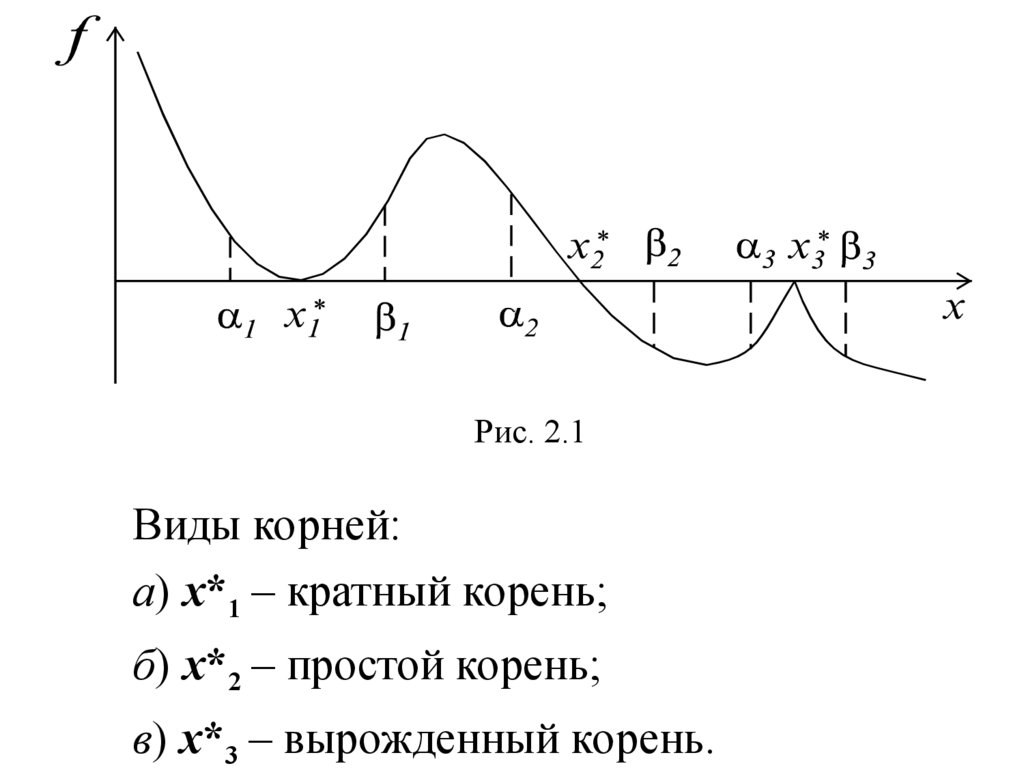
\includegraphics[width=0.7\textwidth]{images/roots-ex.png}
            \caption{Пример корней уравнения}
            \label{fig:roots-example}
        \end{figure}

    \begin{definition}{Основные этапы решения нелинейного уравнения}{def-nonlinear-equation-solve-steps}
        Решение задачи вычисления корней нелинейного уравнения, как правило, осуществляется в два этапа:
        \begin{itemize}
            \item \textbf{Локализация корней}.
            \item \textbf{Итерационное уточнение корней}.
        \end{itemize}
    \end{definition}

    \subsubsection{Локализация корней.}

        \begin{definition}{Отрезок локализации}{def-localization-roots-interval}
            Отрезок $[a, b]$, содержащий только один корень $\overline{x}$, называют \textbf{отрезком локализации}. 
        \end{definition}

        \textbf{Цель этапа локализации}: для каждого из корней указать отрезок локализации (длину отрезка стараются по возможности сделать минимальной).
        
        \vspace{\baselineskip}
        
        Для локализации корней широко применяют построение таблиц значений функции $f(x)$ вида $y_{i} = f(x_{i}), i = 1, 2, \ldots, n$. При этом способе локализации, о наличии на отрезке $[x_{i-1}, x_{i}]$ корня судят по перемене знака функции на концах отрезка.

        \begin{theorem}{Больцано-Коши}{th-Bolzano-Cauchy}
            Пусть функция $f(x)$ непрерывна на отрезке $[a, b]$ и принимает на его концах значения разных знаков, т.е. $f(a) \cdot f(b) < 0$.\\ 
            Тогда отрезок $[a, b]$ содержит по крайне мере один корень уравнения $f(x) = 0$.
        \end{theorem}

    \subsubsection{Итерационное уточнение корней.}
        
        \textbf{Основная идея}: использовать итерационный метод, что позволит построить последовательность $x^{(0)}, x^{(1)}, \ldots, x^{(n)}, \ldots$ приближений к корню $\overline{x}$.

        \begin{definition}{Виды итерационных методов}{def-iterative-method-types}
            Итерационный метод может быть: 
            \begin{itemize}
                \item \textbf{одношаговым}: для вычисления очередного приближения $x^{(n+1)}$ используется только одно предыдущее значение $x^{(n)}$.
                \item \textbf{$k$-шаговым}: для вычисления $x^{(n+1)}$ используется $k$ предыдущих приближений $x^{(n - k + 1)}, x^{(n - k + 2)}, \ldots, x^{(n)}$.
            \end{itemize}
        \end{definition}

        \begin{definition}{Итерационная функция}{def-iterative-function}
            Итерационную последовательность $x^{(0)}, x^{(1)}, \ldots, x^{(n)}, \ldots$ строится через \textbf{итерационную функцию}:
            $$\phi(x^{(0)}) = x^{(1)}$$
            $$\phi(x^{(1)}) = x^{(2)}$$
            $$\ldots$$
            $$\phi(x^{(n-1)}) = x^{(n)}$$
            $$\ldots$$
        \end{definition}

\clearpage
\subsection{Скорость сходимости итерационных методов уточнения решения нелинейного уравнения.}

    \begin{definition}{Скорость сходимости}{def-convergence-rate}
        Говорят, что метод сходится со скоростью \textbf{геометрической прогрессии}, знаменатель которой $q < 1$, если для всех $n$ справедливо:
        $$|x^{(n)} - \overline{x}| \leq c_{0}q^{n}$$

        Пусть существует $\sigma$-окрестность корня $\overline{x}$ такая, что если приближение $x^{(n)}$ принадлежит этой окрестности, то справедлива оценка:
        $$|x^{(n + 1)} - \overline{x}| \leq C|x^{(n)} - \overline{x}|^{p}$$
        где $C > 0$ и $p \geq 1$ - постоянные. Тогда:
        
        \begin{itemize}
            \item Если $p = 1$ и $C < 1$, то метод обладает \textbf{линейной} скоростью сходимости в указанной $\sigma$-окрестности корня.
            \item Если $p > 1$, то метод обладает \textbf{сверхлинейной} скоростью сходимости: при $p = 2$ - \textbf{квадратичной}, при $p = 3$ - \textbf{кубической}.
        \end{itemize}
    \end{definition}

    \begin{lemma}{Связь линейной и геометрической сходимости}{lem-linear-geometric-convergence}
        Пусть одношаговый итерационный метод обладает линейной скоростью сходимости в некоторой $\sigma$-окрестности корня $\overline{x}$. Тогда $\forall x^{(0)} \in [\overline{x} - \sigma, \overline{x} + \sigma]$: 
        \begin{itemize}
            \item Итерационная последовательность $x^{(n)}$ не выходит за пределы  этой окрестности.
            \item Метод сходится со скоростью геометрической прогрессии со знаменателем $q = C$.
        \end{itemize}
        А также имеет место следующая оценка:
        $$|x^{(n)} - \overline{x}| \leq q^{n}|x^{(0)} - \overline{x}| \text{, } n \geq 0$$
    
        \begin{proof}
            $q < 1 \rightarrow x^{(n)} \in [\overline{x} - \sigma, \overline{x} + \sigma]$. Тогда $x^{(n)}$ сходися к $\overline{x}$.

            Справедливость оценки установим через индукцию:\\
            \textbf{При $n = 0$}: 
            $$|x^{(0)} - \overline{x}| \leq |x^{(0)} - \overline{x}|$$
            \textbf{При переходе от $n = m - 1$ к $n = m$}:
            $$|x^{(m)} - \overline{x}| \leq q|x^{(m-1)} - \overline{x}| \leq q^{m}|x^{(0)} - \overline{x}|$$
        \end{proof}
    \end{lemma}


\subsection{Обусловленность задачи решения нелинейных уравнений. Понятие об интервале неопределенности. Правило Гарвика.}

    \subsubsection{Обусловленность задачи решения нелинейных уравнений.}

        Пусть $\overline{x}$ - корень уравнения, $f(x)$ - входные данные для задачи вычисления корня $\overline{x}$, $f^{*}(x)$ - приближенные значения функции.
    
        \begin{definition}{Обусловленность задачи решения нелинейных уравнений}{def-conditionality-nonlinear-equation}
            Нельзя ожидать, что в окрестности корня относительная погрешность $\delta(f^{*}(x))$ окажется малой, например:\\ 
            $$y = \sin(x)$$ 
            в окрестности корней $x = \pi \cdot k$, $k \in \mathbb{Z}$, $\delta(f^{*}(x)) = |x| \cdot \cot(x) \to \infty$. 
        
            \vspace{\baselineskip}
        
            Реально рассчитывать можно лишь на то, что малой окажется абсолютная погрешность вычисления значений функции:
            $$\Delta(f^{*}(x)) \approx |f^{'}(x)| = |\cos(x)|$$
        \end{definition}

    \subsubsection{Понятие об интервале неопределенности. Правило Гарвика.}

        \begin{definition}{Интервал неопределенности}{def-uncertainty-interval}
            Окрестность корня $(\overline{x} - \overline{\varepsilon}, \overline{x} + \overline{\varepsilon})$, в котором невозможно точно определить знак функции $f(x)$: знак вычисленного значения $f^{*}(x)$ может не совпадать со знаком $f(x)$ для $x \in (\overline{x} - \overline{\varepsilon}, \overline{x} + \overline{\varepsilon})$.
        \end{definition}

        \begin{lemma}{Оценка $\overline{\varepsilon}$ для интервала неопределенности}{lem-varepsilon-estimation}
            Пусть корень $\overline{x}$ - простой. Тогда для близких к $\overline{x}$ значений $x$ справедливо приближенное равенство:
            $$f(x) \approx f(\overline{x}) + f^{'}(\overline{x})(x - \overline{x}) = f^{'}(\overline{x})(x - \overline{x})$$
        
            В интервале $(\overline{x} - \overline{\varepsilon}, \overline{x} + \overline{\varepsilon})$, $|f(x)| < \overline{\Delta(f^{*}(x))}$. Следовательно:
            $$|f^{'}(x)(x - \overline{x})| < \overline{\Delta(f^{*}(x))}$$

            Итог: $\overline{x} - \frac{\overline{\Delta(f^{*}(x))}}{|f^{'}(x)|} < x < \overline{x} + \frac{\overline{\Delta(f^{*}(x))}}{|f^{'}(x)|}$ $\rightarrow$ $\overline{\varepsilon} = \frac{1}{|f^{'}(x)|} \cdot \overline{\Delta(f^{*}(x))}$.
        \end{lemma}

        \begin{definition}{Число обусловленности задачи нахождения корня}{def-conditionality-number-root-finding}
            $\nu_{\Delta} = \frac{1}{|f^{'}(\overline{x})|}$ - число обусловленности задачи нахождения корня.
        \end{definition}

        \begin{definition}{Правило Гарвика}{def-garwick-rule}
            $$q^{(n)} = \frac{|x^{(n)} - x^{(n - 1)}|}{|x^{(n - 1)} - x^{(n - 2)}|}$$

            В интервале неопределенности $q^{(n)} > 1$, т.е. начинается разболтка - хаотическое поведение итерационной последовательности.

            \vspace{\baselineskip}

            В этой ситуации вычисления следует прекратить и принять правильное решение. Лучшее из последовательностей приближений к решению становится $x^{(n-1)}$.
        \end{definition}

\clearpage
\subsection{Метод бисекции решения нелинейных уравнений. Скорость сходимости. Критерий окончания.}

    \subsubsection{Описание метода.}

        По сравнению с другими методами метод бисекции сходится довольно медленно. Однако он очень прост и непритязателен; для его применения достаточно, чтобы: 
        \begin{itemize}
            \item Выполнялось неравенство: $f(a)f(b) \leq 0$.
            \item Функция $f(x)$ была непрерывна.
            \item Верно определялся знак функции.
        \end{itemize}
            
        \vspace{\baselineskip}

        Метод гарантирует точность приближения, примерно равную радиусу интервала неопределенности $\overline{\varepsilon}$.

        \begin{definition}{Описание метода}{def-bisection-description}
            Пусть требуется найти с заданной точностью $\varepsilon$ корень $\overline{x}$, а также задан отрезок локализации $[a^{(0)}, b^{(0)}]$ такой, что: $f(a^{(0)}) \cdot f(b^{(0)}) < 0$, тогда:
            $$x^{(0)} = \frac{a^{(0)} + b^{(0)}}{2}$$
            - начальное приближенное значение корня.\\
            Погрешность данного приближения: $\frac{b^{(0)} - a^{(0)}}{2}$

            \vspace{\baselineskip}

            В качестве $[a^{(1)}, b^{(1)}]$ берут тот из отрезков $[a^{(0)}, x^{(0)}]$ и $[x^{(0)}, b^{(0)}]$, на концах которого выполняется условие: $f(a^{(1)})f(b^{(1)}) \leq 0$.\\
            Середина полученного отрезка: 
            $$x^{(1)} = \frac{a^{(1)} + b^{(1)}}{2}$$ 
            - следующее приближение к корню с погрешностью: $\frac{b^{(1)} - a^{(1)}}{2} = \frac{b^{(0)} - a^{(0)}}{2^{2}}$

            \vspace{\baselineskip}

            На очередной $(n + 1)$ итерации происходит следующее:
            \begin{itemize}
                \item Вычисляется $f(x^{(n)})$.
                \item Если $f(a^{(n)})f(x^{(n)}) \leq 0$, то в качестве отрезка локализации $[a^{(n + 1)}, b^{(n + 1)}]$ принимается отрезок $[a^{(n)}, x^{(n)}]$, иначе - $[x^{(n)}, b^{(n)}]$.
                \item Вычисляется $x^{(n + 1)} = \frac{a^{(n + 1)} + b^{(n + 1)}}{2}$.
            \end{itemize}

            \vspace{\baselineskip}

            Если $\frac{b - a}{2^{n + 1}} < \varepsilon$, то останавливаемся: $\overline{x} \approx \frac{a^{(n - 1)} + b^{(n - 1)}}{2}$.
        \end{definition}

    \subsubsection{Скорость сходимости.}

        \begin{lemma}{Скорость сходимости}{lem-bisection-convergence-rate}
            Середина $n$-го отрезка - точка $x^{(n)} = \frac{a^{(n)} + b^{(n)}}{2}$ дает приближение к корню $\overline{x}$, имеющее оценку погрешности:
            $$|x^{(n)} - \overline{x}| \leq \frac{b^{(n)} - a^{(n)}}{2} = \frac{b-a}{2^{n + 1}}$$
        \end{lemma}

        \textbf{Получаем}: метод бисекции сходится со скоростью геометрической прогрессии со знаменателем $q = \frac{1}{2}$.


    \subsubsection{Критерий окончания.}

        \begin{lemma}{Критерий окончания}{lem-bisection-graduation-criteria}
            Итерации следовательно вести до тех пор, пока не будет выполнено неравенство:
            $$(b^{(n)} - a^{(n)}) < 2\varepsilon$$
            При его выполнении можно принять $x^{(n)}$ за приближение к корню с точностью $\varepsilon$.
        \end{lemma}

\clearpage
\subsection{Метод простой итерации. Скорость сходимости. Критерий окончания. Приведение к виду, удобному для итераций.}

    \subsubsection{Описание метода.}

        Геометрически, метод можно представить следующим образом:

        \begin{figure}[H]
            \centering
            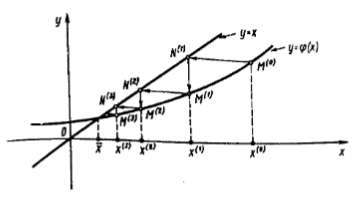
\includegraphics[width=0.7\textwidth]{images/simple-iterations-ex.png}
            \caption{Геометрическое представление метода простых итераций}
            \label{fig:simple-iterations-example}
        \end{figure}

        \begin{definition}{Описание метода}{def-simple-iteration-description}
            \textbf{Основная идея} метода - привести нелинейное уравнение к виду, удобному для итерации:
            $$x = \phi(x)$$
            где функция $\phi(x)$ - итерационная функция.
            
            \vspace{\baselineskip}

            В методе простых итераций $\phi(x) = x - \alpha f(x)$, где $\alpha$ - какая-то константа, $f(x)$ - исходная функция. 
            
            Убедимся, что корень $\phi(x)$ - корень $f(x)$: 
            $$\phi(\overline{x}) = \overline{x} - \alpha f(\overline{x}) = \overline{x}$$

            Пусть $x^{(0)} \in [a, b]$ - начальное приближение корня, тогда:
            $$x^{(1)} = \phi(x^{(0)})$$
            $$x^{(2)} = \phi(x^{(1)})$$
            $$\ldots$$
            $$x^{(n + 1)} = \phi(x^{(n)}) \text{, } n \geq 0$$
            $$\ldots$$
        \end{definition}

    \subsubsection{Скорость сходимости.}

        \begin{figure}[H]
            \centering
            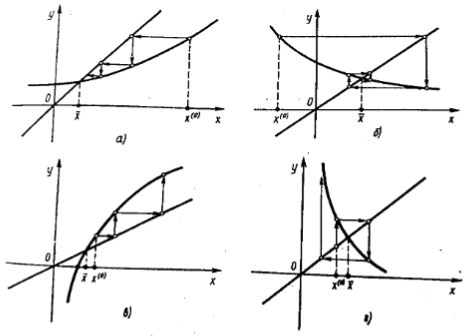
\includegraphics[width=0.7\textwidth]{images/simple-iterations-convergence.png}
            \caption{Сходимость метода простых итераций}
            \label{fig:simple-iterations-example}
        \end{figure}

        Как видно на рисунках, в случаях (а), (б) - метод сходится, а в (в) и (г) - расходится. Это связано с тем, что в (а) и (б) $|\phi^{'}(x)| < 1$, а в (в) и (г) наоборот, $|\phi^{'}(x)| > 1$.

        \begin{theorem}{Об априорной погрешности}{th-simple-iterations-priori-error}
            Пусть в некоторой $\sigma$-окрестности корня $\overline{x}$ функция $\phi(x)$ дифференцируема и удовлетворяет неравенству:
            $$|\phi^{'}(x)| \leq q$$
            где $0 \leq q < 1$ - постоянная.\\

            Тогда $\forall x^{(0)} \in [\overline{x} - \sigma, \overline{x} + \sigma]$ итерационная последовательность:
            \begin{itemize}
                \item Не выходит за пределы этой окрестности.
                \item Метод сходится со скоростью геометрической прогрессии. 
            \end{itemize}
            А также справедлива следующая оценка погрешности:
            $$|x^{(n)} - \overline{x}| \leq q^{n}|x^{(0)} - \overline{x}|$$

            \begin{proof}
                По определению:
                $$x^{(n + 1)} = \phi(x^{(n)})$$
                $$\overline{x} = \phi(\overline{x})$$

                Тогда:
                $$x^{(n + 1)} - \overline{x} = \phi(x^{(n)}) - \phi(\overline{x}) = \phi^{'}(\xi^{(n)})(x^{(n)} - \overline{x})$$
                Причем:
                $$\xi^{(n)} \in [x^{(n)}, \overline{x}]$$

                Значит:
                $$|x^{(n+1)} - \overline{x}| = |\phi^{'}(\xi^{(n)})| \cdot |x^{(n)} - \overline{x}| \leq q \cdot |x^{(n)} - \overline{x}|$$
            
                Следовательно: интерполяционная последовательность $x^{(0)}, x^{(1)}, \ldots, x^{(k)}, \ldots$ сходится линейно к $\overline{x}$ (отсюда получаем, что последовательность сходится со скоростью геометрической последовательности со знаменателем $q$).
            \end{proof}

        \end{theorem}

        \textbf{Априорные оценки} погрешности позволяют еще до вычислений дать некоторое заключение о качестве метода.

    \subsubsection{Критерий окончания.}
        
        \begin{theorem}{Об апостериорной погрешности}{th-simple-iterations-posteriori-error}
            Пусть в некоторой $\sigma$-окрестности корня $\overline{x}$ функция $\phi(x)$ дифференцируема и удовлетворяет неравенству:
            $$|\phi^{'}(x)| \leq q$$
            где $0 \leq q < 1$ - постоянная.\\

            Тогда $\forall x^{(0)} \in [\overline{x} - \sigma, \overline{x} + \sigma]$ верна следующая апостериорная оценка погрешности:
            $$|x^{(n)} - \overline{x}| \leq \frac{q}{1 - q} |x^{(n)} - x^{(n - 1)}| \text{, } n \geq 1$$

            \begin{proof}
                $$x^{(n)} - \overline{x} = \phi(x^{(n - 1)}) - \phi(\overline{x}) = \phi^{'}(\xi^{(n)})(x^{(n - 1)} - \overline{x})$$

                Пусть: 
                $$\phi^{'}(\xi^{n}) = \alpha^{(n+1)}$$

                Тогда:
                $$x^{(n)} - \overline{x} = \alpha^{(n+1)}(x^{(n+1)} - \overline{x})$$
                $$\alpha^{(n + 1)}(x^{(n - 1)} - x^{(n)} + x^{(n)} - \overline{x}) = \alpha^{(n + 1)}(x^{(n - 1)} - x^{(n)}) + \alpha^{(n + 1)}(x^{(n)} - \overline{x})$$
                
                Значит:
                $$|x^{(n)} - \overline{x}| \leq |\alpha^{(n + 1)}| \cdot |x^{(n - 1)} - x^{(n)}| + |\alpha^{(n + 1)}| \cdot |x^{(n)} - \overline{x}|$$

                $$(1 - |\alpha^{(n + 1)}|) \cdot |x^{(n)} - \overline{x}| \leq |\alpha^{(n + 1)}| \cdot |x^{(n - 1)} - x^{(n)}|$$
                $$|x^{(n)} - \overline{x}| \leq \frac{|\alpha^{(n + 1)}|}{1 - |\alpha^{n + 1}|} \cdot |x^{(n - 1)} - x^{(n)}|$$

                Т.к. $$\begin{cases} 
                       |\alpha^{(n + 1)}| \leq q \\
                       1 - |\alpha^{(n + 1)}| \geq 1 - q
                       \end{cases}$$ то:
                $$|x^{(n)} - \overline{x}| \leq \frac{q}{1-q} \cdot |x^{(n - 1)} - x^{(n)}|$$
            \end{proof}
        \end{theorem}

        Если величина $q$ известна, то неравенство выше дает эффективный метод контроля погрешности и можно сформулировать следующий критерий окончания итерационного процесса.

        \begin{consequence}{Критерий остановки}{con-simple-iterations-graduation-criteria}
            Вычисления следует вести до выполнения неравенства:
            $$\frac{q}{1 - q}|x^{(n)} - x^{(n - 1)}| < \varepsilon$$
            
            или равносильному ему неравенства:
            $$|x^{(n)} - x^{(n - 1)}| < \frac{1-q}{q} \varepsilon$$
        \end{consequence}

        Использование данного критерия окончания требует знание величины $q$. Чтобы избавиться от нее, оценим $q$.

        \begin{lemma}{Оценка величины $q$}{lem-estimating-value-q}
            $$|x^{(n)} - x^{(n - 1)}| < \frac{1 - \overline{\alpha^{(n)}}}{\overline{\alpha^{(n)}}} \varepsilon$$

            \begin{proof}
                Заметим, что в малой окрестности корня величина производной $\phi^{'}(x)$ практически постоянна: 
                $$\phi^{'}(x) \approx \phi^{'}(\overline{x})$$

                Тогда величину $\alpha^{(n)} = \phi^{'}(\xi^{(n - 1)})$ можно приближенно заменить на $\phi^{'}(\overline{x})$.\\
                Следовательно:
                $$x^{(n)} - x^{(n - 1)} = \phi(x^{(n - 1)}) - \phi(x^{(n - 2)}) = \phi^{'}(\overline{\xi^{(n)}})(x^{(n - 1)} - x^{(n - 2)})$$
                где: $\overline{\xi^{(n)}} \in [x^{(n - 1)}, x^{(n - 2)}]$.\\

                Тогда:
                $$\overline{\alpha^{(n)}} = \frac{x^{(n)} - x^{(n - 1)}}{x^{(n - 1)} - x^{(n - 2)}} = \phi^{'}(\overline{\xi^{(n)}}) \approx \phi^{'}(\overline{x})$$
            
                Таким образом: можно положить $\alpha^{(n)} \approx \overline{\alpha^{(n)}}$.
                $$|x^{(n)} - x^{(n - 1)}| < |\frac{1 - \overline{\alpha^{(n)}}}{\overline{\alpha^{(n)}}}| \varepsilon$$
            \end{proof}
        \end{lemma}

    \subsubsection{Приведение к виду, удобного для итераций.}
        
        \begin{theorem}{Приведение к виду, удобного для итераций}{th-bringing-to-form-convenient-for-iteration}
            Пусть $f(x) \in C^{1}[a, b]$, причем $f^{'}(x) \geq 0$.\\ 
            Тогда $\exists m, M \in \mathbb{R} \text{: } 0 < m \leq f^{'}(x) \leq M$, $x \in [a, b]$.\\
            Тогда при:
            $$\alpha_{\text{opt}} = \frac{2}{m + M}$$
            $|\phi^{'}(x)| \leq q < 1$, причем значение $q$ - минимально.


            \begin{proof}
                Т.к. $m \leq \phi^{'}(x) \leq M$, то:
                $$1 - \alpha M \leq \phi^{'}(x) \leq 1 - \alpha m$$

                В соотношении:
                $$|\phi^{'}(x) \leq q|$$
                Величина $q$ должна быть минимальна.\\

                Следовательно:
                $$|\phi^{'}(x) \leq \max_{\alpha}|\{|1 - \alpha M| \text{, } |1 - \alpha m|\}$$

                Получаем:
                $$1 - \alpha m = -1 + \alpha M$$

                Отсюда:
                $$\alpha_{\text{opt}} = \frac{2}{m + M}$$
            \end{proof}
        \end{theorem}

\clearpage
\subsection{Метод Ньютона решения нелинейных уравнений. Вывод итерационной формулы метода Ньютона.}

    Расчетную формулу метода можно получить, используя различные подходы. 

    \begin{definition}{Метод касательных}{def-newton-tangent-method}
        \textbf{Шаги алгоритма:}
        \begin{itemize}
            \item Пусть $x^{(0)} \in [a, b]$ - начальное приближение к корню $\overline{x}$.
            \item Выбираем точку $M(x^{(0)}, f(x^{(0)}))$.
            \item Строим через $M$ касательную к графику $f(x)$.
            \item Пересечение с осью $Ox$ - следующее приближение $x^{(1)}$.
        \end{itemize}
        Продолжая этот процесс далее, получим последовательность $x^{(0)}, x^{(1)}, \ldots, x^{(n)}, \ldots$ приближений к корню $\overline{x}$.
            
        \vspace{\baselineskip}

        Уравнение касательной, проведенной к графику функции $y = f(x)$ в точке $(x^{(n)}, f(x^{(n)}))$, имеет вид:
        $$y = f(x^{(n)}) + f^{'}(x^{(n)})(x - x^{(n)})$$

        Полагая в равенстве $y = 0$ и $f^{'}(x^{(n)}) \neq 0$, получаем:
        $$0 = f(x^{(n)}) + f^{'}(x^{(n)})(x^{(n + 1)} - x^{(n)})$$

        \textbf{Расчетная формула}:
        $$x^{(n + 1)} = x^{(n)} - \frac{f(x^{(n)})}{f^{'}(x^{(n)})} \text{, } n \geq 0$$
    \end{definition}

    \begin{figure}[H]
        \centering
        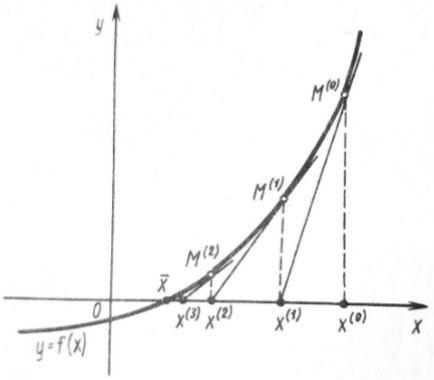
\includegraphics[scale=0.7]{images/newton-tangent-method-ex.png}
        \caption{Метод касательных}
        \label{fig:newton-tangent-method}
    \end{figure}

    С более общих позиций \textbf{метод Ньютона} можно рассматривать как \textbf{итерационный метод}, использующий специальную линеаризацию задачи.

    \begin{definition}{Метод линеаризации}{def-newton-linearization-method}
        Пусть приближение $x^{(n)}$ уже получено. Представим функцию в окрестности точки $x^{(n)}$ по формуле Тейлора:
        $$f(x) = f(x^{(n)}) + f^{'}(x^{(n)})(x - x^{(n)}) + \frac{f^{''}(\xi)}{2}(x - x^{(n)})^{2}$$
        где: $\xi \in [x, x^{(n)}]$
        
        \vspace{\baselineskip}

        Заменяя в уравнении $f(x) = 0$ функцию $f(x)$, получаем:
        $$f(x^{(n)}) + f^{'}(x^{(n)})(x - x^{(n)}) = 0$$

        Принимая решение уравнения за новое приближение $x^{(n + 1)}$, приходим к формуле:
        $$x^{(n + 1)} = x^{(n)} - \frac{f(x^{(n)})}{f^{'}(x^{(n)})}$$
    \end{definition}

\clearpage
\subsection{Априорная погрешность метода Ньютона.}

    \begin{theorem}{Об априорной погрешности}{th-newton-priori-error}
        Пусть $f(x) \in C^{2}[a, b]$ - отрезок локализации и $\overline{x}$ - простой корень. Тогда сущствует некоторая $\sigma$-окрестность: $(\overline{x} - \sigma, \overline{x} + \sigma)$: $\forall x^{(0)} \in (\overline{x} - \sigma, \overline{x} + \sigma)$, итерационная последовательность не выходит из этой окрестности и справедлива оценка:
        $$|x^{(n + 1)} - \overline{x}| \leq C|x^{(n)} - \overline{x}|^{2} \text{, } n \geq 0$$
        где: $C = \sigma^{-1}$.

        \begin{proof}
            Т.к. $f \in C^{2}[a, b]$, то: 
            $$\exists \alpha, \beta > 0 \text{: } \begin{cases} 0 < \alpha \leq |f^{'}(x)| \\ |f^{''}(x)| < \beta \end{cases}$$

            Тогда:
            \begin{enumerate}
                \item $0 = f(x^{(n)}) + f^{'}(x^{(n)})(x^{(n + 1)} - x^{(n)})$
                \item $f(x) = f(x^{(n)}) + f^{'}(x^{(n)})(x - x^{(n)}) + \frac{f^{''}(\xi)}{2}(x - x^{(n)})^{2}$
            \end{enumerate}

            Подставим во второе уравнение $x = \overline{x}$: $f(\overline{x}) = 0$
            $$0 = f(x^{(n)}) + f^{'}(x^{(n)})(\overline{x} - x^{(n)}) + \frac{f^{''}(\xi)}{2}(\overline{x} - x^{(n)})$$

            Вычтем из перовго уравнения второе:
            $$0 = f^{'}(x^{(n)})(\overline{x} - x^{(n)} - x^{(n + 1)} + x^{(n)}) + \frac{f^{''}(\xi)}{2}(\overline{x} - x^{(n)})^{2}$$
            $$f^{'}(x^{(n)})(x^{(n + 1)} - \overline{x}) = \frac{f^{''}(\xi)}{2}(x^{(n)} - \overline{x})^{2}$$
            $$\alpha |x^{(n + 1)} - \overline{x}| \leq \frac{\beta}{2}|x^{(n)} - \overline{x}|^{2}$$
            $$|x^{(n + 1)} - \overline{x}| \leq \frac{\beta}{2\alpha}|x^{(n)} - \overline{x}|^{2}$$

            Возьмем за $\sigma = \frac{2\alpha}{\beta}$:
            $$|x^{(n + 1)} - \overline{x}| \leq \sigma^{-1} |x^{(n)} - \overline{x}|^{2}$$
        \end{proof}
    \end{theorem}

    \begin{consequence}{Априорной погрешности}{con-priori-error}
        Априорная оценка погрешности для метода Ньютона:
        $$|x^{(n)} - \overline{x}| \leq \sigma q^{2^{n}} \text{, } n \geq 0$$
        где: $q = \sigma^{-1}|x^{(0)} - \overline{x}|$.
    
        \begin{proof}
            По индукции.
        \end{proof}
    \end{consequence}

\clearpage
\subsection{Апостериорная оценка погрешности (критерий окончания). Правило выбора начального приближения на отрезке локализации корня, гарантирующего сходимость метода.}

    \begin{theorem}{Об апостериорная погрешность}{th-newton-posteriori-error}
        Пусть $x^{(n)} \in (\overline{x} - \frac{\sigma}{2}, \overline{x} + \frac{\sigma}{2})$, тогда: в условиях теоремы об априорной погрешности:
        $$|x^{(n)} - \overline{x}| \leq |x^{(n)} - x^{(n - 1)}|$$
    
        \begin{proof}
            $$2|x^{(n)} - \overline{x}| \leq 2 \sigma^{-1} |x^{(n - 1)} - \overline{x}|^{2}$$
            $$2 \cdot \sigma^{-1} |x^{(n - 1)} - \overline{x}| \cdot |x^{(n - 1)} - \overline{x}| \leq |x^{(n-1)} - \overline{x}|$$
            $$|x^{(n-1)} - x^{(n)} + x^{(n)} - \overline{x}| \leq |x^{(n-1)} - x^{(n)}| + |x^{(n)} - \overline{x}|$$
            $$|x^{(n)} - \overline{x}| \leq |x^{(n-1)} - x^{(n)}|$$
        \end{proof}
    \end{theorem}

    \begin{consequence}{Критерий остановки}{con-newton-graduation-criteria}
        $$|x^{(n)} - x^{(n - 1)}| < \varepsilon$$
        где: $\varepsilon$ - заданная точность.
    \end{consequence}

    В качестве начального приближения можно выбрать \textbf{не любую} точку из $[a, b]$. Иначе: касательная может пересечь $Ox$ вне интервала.

    \begin{theorem}{Критерий выбора начального приближения}{th-newton-choosing-initial-approximation}
        Пусть $f(x) \in C^{2}[a, b]$ и $f^{'}(x)$ и $f^{''}(x)$ - знакопостоянны.\\
        Тогда итерационная последовательность метода Ньютона сходится, если в качестве $x^{(0)}$ выбрать точку такую, что:
        $$f(x^{(0)})f^{''}(x^{(0)}) > 0$$

        Таким образом, метод Ньютона \textbf{обладает} в общем случае только \textbf{локальной сходимостью}.
    \end{theorem}

\clearpage
\subsection{Модификации метода Ньютона. Упрощенный метод Ньютона. Метод хорд.}

    \begin{definition}{Упрощенный метод Ньютона}{def-simplified-newton}
        Исходная формула Ньютона:
        $$x^{(n + 1)} = x^{(n)} - \frac{f(x^{(n)})}{f^{'}(x^{(n)})} \text{, } n \geq 0$$

        Формула упрощенного Ньютона: $f^{'}(x^{(n)}) \approx f^{'}(x^{(0)})$
        $$x^{(n + 1)} = x^{(n)} - \frac{f(x^{(n)})}{f^{'}(x^{(0)})} \text{, } n \geq 0$$
   
        Т.е:
        \begin{itemize}
            \item В точке $(x^{(0)}, f(x^{(0)}))$ к графику функции $y = f(x)$ проводится касательная $l_{0}$.
            \item За приближение $x^{(1)}$ принимается абцисса точки пересечения $l_{0}$ с осью $Ox$.
            \item Каждое следующее приближение $x^{(n + 1)}$ получается как абцисса точки пересечения с осью $Ox$ прямой, проходящей через точку $M^{(n)}(x^{(n)}, f(x^{(n)}))$ и параллельной касательной $l_{0}$.
        \end{itemize}

        \vspace{\baselineskip}

        Данный метод можно рассматривать как \textbf{метод простой итерации} с формулой:
        $$\phi(x) = x - \frac{f(x)}{f^{'}(x^{(0)})}$$

        \vspace{\baselineskip}

        \textbf{Скорость сходимоти} данного метода - \textbf{линейная}.
    \end{definition}

    \begin{figure}[H]
        \centering
        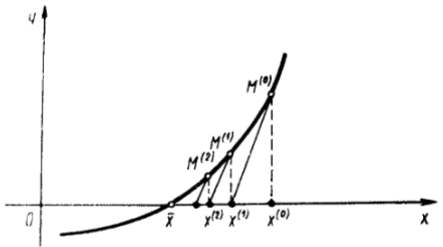
\includegraphics[scale=0.7]{images/simplified-newton-ex.png}
        \caption{Упрощенный метод Ньютона}
        \label{fig:simplified-newton-method}
    \end{figure}

    \begin{definition}{Метод хорд}{def-chord-method}
        По определению производной:
        $$f^{'}(x^{(n)}) = \frac{f(z^{(n)}) - f(x^{(n)})}{z^{(n)} - x^{(n)}} \text{, при: } z^{(n)} \to x^{(n)}$$
        
        Тогда вместо:
        $$x^{(n + 1)} = x^{(n)} - \frac{f(x^{(n)})}{f^{'}(x^{(n)})}$$
        Фиксируем: $f^{'}(x^{(n)}) = \frac{f(c) - f^{'}(x^{(n)})}{c - x^{(n)}}$

        Итоговая формула:
        $$x^{(n + 1)} = x^{(n)} - \frac{c - x^{(n)}}{f(c) - f(x^{(n)})} \cdot f(x^{(n)}) \text{, } n \geq 0$$
        
        где $c$ - фиксированная точка, расположенная в окрестности простого корня $\overline{x}$.
    
        \vspace{\baselineskip}
    
        Очередное приближение $x^{(n + 1)}$ получается здесь как абцисса точки пересечения с осью $Ox$ прямой, проходящей через расположенные на графике функции $y = f(x)$ точки $M(c, f(c))$ и $M^{(n)}(x^{(n)}, f(x^{(n)}))$
    
        \vspace{\baselineskip}
    
        Метод можно рассматривать как \textbf{итерационный}, с формулой:
        $$\phi(x) = x - \frac{c - x}{f(c) - f(x)}f(x)$$
    
        \vspace{\baselineskip}

        \textbf{Скорость сходимости} данного метода - \textbf{линейная}.
    \end{definition}

    \begin{figure}[H]
        \centering
        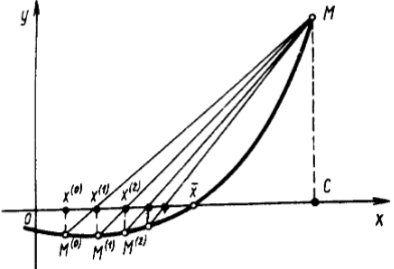
\includegraphics[scale=0.7]{images/chord-method-ex.png}
        \caption{Метод хорд}
        \label{fig:chord-method}
    \end{figure}

\clearpage
\subsection{Модификации метода Ньютона. Метод секущих. Скорость сходимости метода секущих.}

    \begin{definition}{Метод секущих}{def-secant-method}
        Замена $f^{'}(x^{(n)})$ на $\frac{f(x^{(n + 1)}) - f(x^{(n)})}{x^{(n - 1)} - x^{(n)}}$ приводит к расчетной формуле:
        $$x^{(n + 1)} = x^{(n)} - \frac{x^{(n - 1)} - x^{(n)}}{f(x^{(n - 1)}) - f(x^{(n)})} f(x^{(n)}) \text{, } n \geq 1$$

        Данный метод является \textbf{двухшаговым}.
    
        \vspace{\baselineskip}

        Очередное приближение $x^{(n + 1)}$ получается как абцисса точки пересечения с осью $Ox$ секущей, соединяющей точки $M^{(n - 1)}(x^{(n - 1)}, f(x^{(n - 1)}))$ и $M^{(n)}(x^{(n)}, f(x^{(n)}))$, графика функции $f(x)$.
    \end{definition}

    \begin{figure}[H]
        \centering
        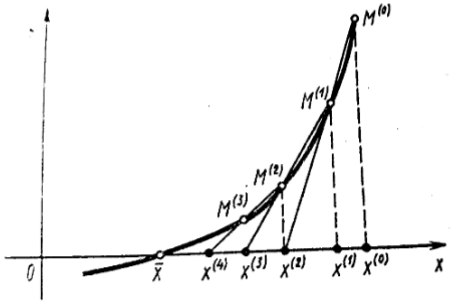
\includegraphics[scale=0.7]{images/secant-method-ex.png}
        \caption{Метод секущих}
        \label{fig:secant-method}
    \end{figure}

    \begin{lemma}{Скорость сходимости метода секущих}{lem-secant-method-convergence-rate}
        Метод секущих сходится с порядком $p = \frac{1 + \sqrt{5}}{2} \approx 1.618$, т.е. для $n \geq 1$ справедлива оценка:
        $$|x^{(n + 1)} - \overline{x}| \leq c|x^{(n)} - \overline{x}|^{p} \text{, } p = \frac{1 + \sqrt{5}}{2}$$

        \begin{itemize}
            \item Одная итерация метода секущих требует только одного нового вычисления $f(x)$.
            \item Метод Ньютона требует двух вычислений: $f(x)$ и $f^{'}(x)$
            \item Трудоемкость двух итераций метода секущих $\sim$ трудоемкость одной итерации метода Ньютона.
            \item Две итерации метода секущих дают порядок $p^{2} \approx 2.618 > 2$ $\rightarrow$ его можно расценивать как \textbf{более быстрый}.
        \end{itemize}
    \end{lemma}

    Метод \textbf{обладает} только \textbf{локальной сходимостью}: он \textbf{требует} выбора \textbf{двух близких к корню} начальных приближений $x^{(0)}$ и $x^{(1)}$.

\clearpage
\subsection{Решение СЛАУ. Постановка задачи.}



\clearpage
\subsection{Решение СЛАУ. Определение понятия нормы вектора. Абсолютная и относительная погрешности вектора.}

\clearpage
\subsection{Решение СЛАУ. Определение понятия нормы матрицы, подчиненной норме вектора. Геометрическая интерпретация нормы матрицы.}

\clearpage
\subsection{Обусловленность задачи решения СЛАУ для приближенно заданной правой части. Количественная мера обусловленности СЛАУ. Геометрическая интерпретация числа обусловленности.}

\clearpage
\subsection{Обусловленность задачи решения СЛАУ для приближенно заданных матрицы и правой части.}

\clearpage
\subsection{Метод Гаусса решения СЛАУ. Схема единственного деления. LU – разложение. Свойства метода.}

\clearpage
\subsection{Метод Гаусса решения СЛАУ. Схемы частичного и полного выбора ведущих элементов. Свойства методов.}

\clearpage
\subsection{Применение метода Гаусса к решению задач линейной алгебры. Вычисление решений системы уравнений с несколькими правыми частями.}

\clearpage
\subsection{Применение метода Гаусса к решению задач линейной алгебры. Вычисление обратной матрицы.}

\clearpage
\subsection{Применение метода Гаусса к решению задач линейной алгебры. Вычисление выражений вида v = CWw. Вычисление определителя матрицы.}

\clearpage
\subsection{Метод Холецкого решения СЛАУ с симметричной положительно определенной матрицей. Свойства метода.}

\clearpage
\subsection{Метод прогонки решения СЛАУ с трехдиагональными матрицами. Свойства метода.}

\clearpage
\subsection{Постановка задачи приближения функций. Приближение функций обобщенными многочленами.}

\clearpage
\subsection{Приближение методом интерполяции. Интерполяция обобщенными многочленами.}

\clearpage
\subsection{Понятия линейно-независимой системы функций на заданном множестве точек. Теорема о существовании единственного решения задачи интерполяции.}

\clearpage
\subsection{Понятия ортогональной системы функций на заданном множестве точек. Утверждение о существовании единственного решения задачи интерполяции с помощью ортогональной системы функций. Решение задачи интерполяции для этого случая.}

\clearpage
\subsection{Полиномиальная интерполяция. Интерполяционный многочлен в форме Лагранжа.}

\clearpage
\subsection{Погрешность полиномиальной интерполяции.}

\clearpage
\subsection{Интерполяционный многочлен с кратными узлами. Погрешность интерполяции с кратными узлами.}

\clearpage
\subsection{Минимизация оценки погрешности интерполяции. Многочлены Чебышева и их свойства. Применение для решения задачи минимизации погрешности.}

\clearpage
\subsection{Интерполяционная формула Ньютона для неравных промежутков. Разделенные разности и их свойства.}

\clearpage
\subsection{Вывод формулы Ньютона для неравных промежутков с помощью разделенных разностей.}

\clearpage
\subsection{Интерполяционная формула Ньютона для равных промежутков. Конечные разности и их связь с разделенными разностями.}

\clearpage
\subsection{Вывод формул Ньютона для интерполирования вперед и назад.}

\clearpage
\subsection{Проблемы глобальной полиномиальной интерполяции. Интерполяция сплайнами. Определение сплайна. Интерполяционный сплайн.}

\clearpage
\subsection{Интерполяция сплайнами. Построение локального кубического интерполяционного сплайна.}

\clearpage
\subsection{Интерполяция сплайнами. Глобальные способы построения кубического интерполяционного сплайна.}

\section{Интерполяция}


\section{Дифференцирование и интегрирование}

\section{Список вопросов}
\begin{enumerate}
    \item Предмет вычислительной математики. Метод и задачи вычислительной математики в терминах функционального анализа. 
    \item Источники и классификация погрешностей результатов численного решения задач. Приближенные числа. Абсолютная и относительная погрешности. Правила записи приближенных чисел. 
    \item Погрешности арифметических операций над приближенными числами. Погрешность функции одной и многих переменных. 
    \item Корректность вычислительной задачи. Примеры корректных и некорректных задач. 
    \item Обусловленность вычислительной задачи. Примеры хорошо и плохо обусловленных задач. 
    \item Вычислительные алгоритмы. Корректность и обусловленность вычислительных алгоритмов. 
    \item Постановка задачи решения нелинейных уравнений. Основные этапы решения задачи. 
    \item Скорость сходимости итерационных методов уточнения решения нелинейного уравнения. 
    \item Обусловленность задачи решения нелинейных уравнений. Понятие об интервале неопределенности. Правило Гарвика. 
    \item Метод бисекции решения нелинейных уравнений. Скорость сходимости. Критерий окончания. 
    \item Метод Ньютона решения нелинейных уравнений. Вывод итерационной формулы метода Ньютона. 
    \item Априорная оценка погрешности метода Ньютона (теорема о скорости сходимости). 
    \item Апостериорная оценка погрешности (критерий окончания). Правило выбора начального приближения на отрезке локализации корня, гарантирующего сходимость метода. 
    \item Модификации метода Ньютона. Упрощенный метод Ньютона. Метод хорд. 
    \item Модификации метода Ньютона. Метод секущих. Скорость сходимости метода секущих. 
    \item Решение систем линейных алгебраических уравнений. Постановка задачи. 
    \item Решение систем линейных алгебраических уравнений. Определение понятия нормы вектора. Абсолютная и относительная погрешности вектора. 
    \item Решение систем линейных алгебраических уравнений. Определение понятия нормы матрицы, подчиненной норме вектора. Геометрическая интерпретация нормы матрицы. 
    \item Обусловленность задачи решения системы линейных алгебраических уравнений для приближенно заданной правой части. Количественная мера обусловленности системы линейных алгебраических уравнений. Геометрическая интерпретация числа обусловленности. 
    \item Обусловленность задачи решения системы линейных алгебраических уравнений для приближенно заданных матрицы и правой части. 
    \item Метод Гаусса решения систем линейных алгебраических уравнений. Схема единственного деления. LU – разложение. Свойства метода. 
    \item Метод Гаусса решения систем линейных алгебраических уравнений. Схемы частичного и полного выбора ведущих элементов. Свойства методов. 
    \item Применение метода Гаусса к решению задач линейной алгебры. Вычисление решений системы уравнений с несколькими правыми частями. 
    \item Применение метода Гаусса к решению задач линейной алгебры. Вычисление обратной матрицы. 
    \item Применение метода Гаусса к решению задач линейной алгебры. Вычисление выражений вида v = CWw. Вычисление определителя матрицы. 
    \item Метод Холецкого решения систем линейных алгебраических уравнений с симметричной положительно определенной матрицей. Свойства метода. 
    \item Метод прогонки решения систем линейных алгебраических уравнений с трехдиагональными матрицами. Свойства метода. 
    \item Постановка задачи приближения функций. Приближение функций обобщенными многочленами. 
    \item Приближение методом интерполяции. Интерполяция обобщенными многочленами. 
    \item Понятия линейно-независимой системы функций на заданном множестве точек. Теорема о существовании единственного решения задачи интерполяции. 
    \item Понятия ортогональной системы функций на заданном множестве точек. Утверждение о существовании единственного решения задачи интерполяции с помощью ортогональной системы функций. Решение задачи интерполяции для этого случая. 
    \item Полиномиальная интерполяция. Интерполяционный многочлен в форме Лагранжа. 
    \item Погрешность полиномиальной интерполяции. 
    \item Интерполяционный многочлен с кратными узлами. Погрешность интерполяции с кратными узлами. 
    \item Минимизация оценки погрешности интерполяции. Многочлены Чебышева и их свойства. Применение для решения задачи минимизации погрешности. 
    \item Интерполяционная формула Ньютона для неравных промежутков. Разделенные разности и их свойства. 
    \item Вывод формулы Ньютона для неравных промежутков с помощью разделенных разностей.  
    \item Интерполяционная формула Ньютона для равных промежутков. Конечные разности и их связь с разделенными разностями. 
    \item Вывод формул Ньютона для интерполирования вперед и назад. 
    \item Проблемы глобальной полиномиальной интерполяции. Интерполяция сплайнами. Определение сплайна. Интерполяционный сплайн. 
    \item Интерполяция сплайнами. Построение локального кубического интерполяционного сплайна. 
    \item Интерполяция сплайнами. Глобальные способы построения кубического интерполяционного сплайна. 
    \item Простейшие формулы численного дифференцирования. Вычисление первой производной. Погрешность формул. 
    \item Простейшие формулы численного дифференцирования. Вычисление второй производной. Погрешность формул. 
    \item Общий подход к выводу формул численного дифференцирования с помощью интерполяционного многочлена. 
    \item Обусловленность формул численного дифференцирования. 
    \item Численное интегрирование. Простейшие квадратурные формулы. Формула прямоугольников. Погрешность формулы. 
    \item Численное интегрирование. Простейшие квадратурные формулы. Формула трапеций. Погрешность формулы. 
    \item Численное интегрирование. Простейшие квадратурные формулы. Формула Симпсона. Погрешность формулы. 
    \item Апостериорные оценки погрешности квадратурных формул. Правило Рунге.
\end{enumerate}

\end{document}